\documentclass[12pt]{article}
 
\usepackage[margin=1in]{geometry} 
\usepackage{amsmath,amsthm,amssymb}
\usepackage{graphicx}
\usepackage{attachfile}

\graphicspath{ {images/} }
 

\begin{document}
 
% --------------------------------------------------------------
%                         Start here
% --------------------------------------------------------------
 
\title{\Huge \textbf{Tým xhricma00 varianta vv-BVS}}

\author{\bf Marek Hric \\
\bf xhricma00
\and Mikuláš Lešiga\\
 xlesigm00
\and Roman Andraščík \\
 xandrar00
\and Adam Veselý \\ 
xvesela00
}

\maketitle
\bigskip
\begin{center}
 \Large \textbf{Rozdelenie bodov}  \normalsize
 \\ 
\medskip
xhricma00: 25\% \\
xlesigm00: 25\% \\
xandrar00: 25\% \\
xvesela00: 25\%  \\
\bigskip
 \Large \textbf{Rozšírenia} \normalsize
\\
\medskip
ORELSE\\
UNREACHABLE\\
BOOLTHEN\\
FOR\\
WHILE\\
FUNEXP\\
\end{center}

\newpage

\noindent \Large \textbf{Rozdelenie prace :} \\
\noindent\makebox[\linewidth]{\rule{\textwidth}{0.4pt}}
\newline \\
\indent \large Marek Hric : \normalsize
\paragraph{Lorem ipsum dolor sit amet, consectetur adipiscing elit, sed do eiusmod tempor incididunt ut labore et dolore magna aliqua. Ut enim ad minim veniam, quis nostrud exercitation ullamco laboris nisi ut aliquip ex ea commodo consequat. Duis aute irure dolor in reprehenderit in voluptate velit esse cillum dolore eu fugiat nulla pariatur. Excepteur sint occaecat cupidatat non proident, sunt in culpa qui officia deserunt mollit anim id est laborum \newline \\} 
\large Mikuláš Lešiga :
\normalsize
\paragraph{Lorem ipsum dolor sit amet, consectetur adipiscing elit, sed do eiusmod tempor incididunt ut labore et dolore magna aliqua. Ut enim ad minim veniam, quis nostrud exercitation ullamco laboris nisi ut aliquip ex ea commodo consequat. Duis aute irure dolor in reprehenderit in voluptate velit esse cillum dolore eu fugiat nulla pariatur. Excepteur sint occaecat cupidatat non proident, sunt in culpa qui officia deserunt mollit anim id est laborum \newline \\}
\large Roman Andraščík :
\normalsize
\paragraph{Lorem ipsum dolor sit amet, consectetur adipiscing elit, sed do eiusmod tempor incididunt ut labore et dolore magna aliqua. Ut enim ad minim veniam, quis nostrud exercitation ullamco laboris nisi ut aliquip ex ea commodo consequat. Duis aute irure dolor in reprehenderit in voluptate velit esse cillum dolore eu fugiat nulla pariatur. Excepteur sint occaecat cupidatat non proident, sunt in culpa qui officia deserunt mollit anim id est laborum \newline \\}
\large Adam Veselý :
\normalsize
\paragraph{Lorem ipsum dolor sit amet, consectetur adipiscing elit, sed do eiusmod tempor incididunt ut labore et dolore magna aliqua. Ut enim ad minim veniam, quis nostrud exercitation ullamco laboris nisi ut aliquip ex ea commodo consequat. Duis aute irure dolor in reprehenderit in voluptate velit esse cillum dolore eu fugiat nulla pariatur. Excepteur sint occaecat cupidatat non proident, sunt in culpa qui officia deserunt mollit anim id est laborum \newline \\}
 
\newpage

\noindent \Large \textbf{Diagram konečného automatu :}
\newline \\

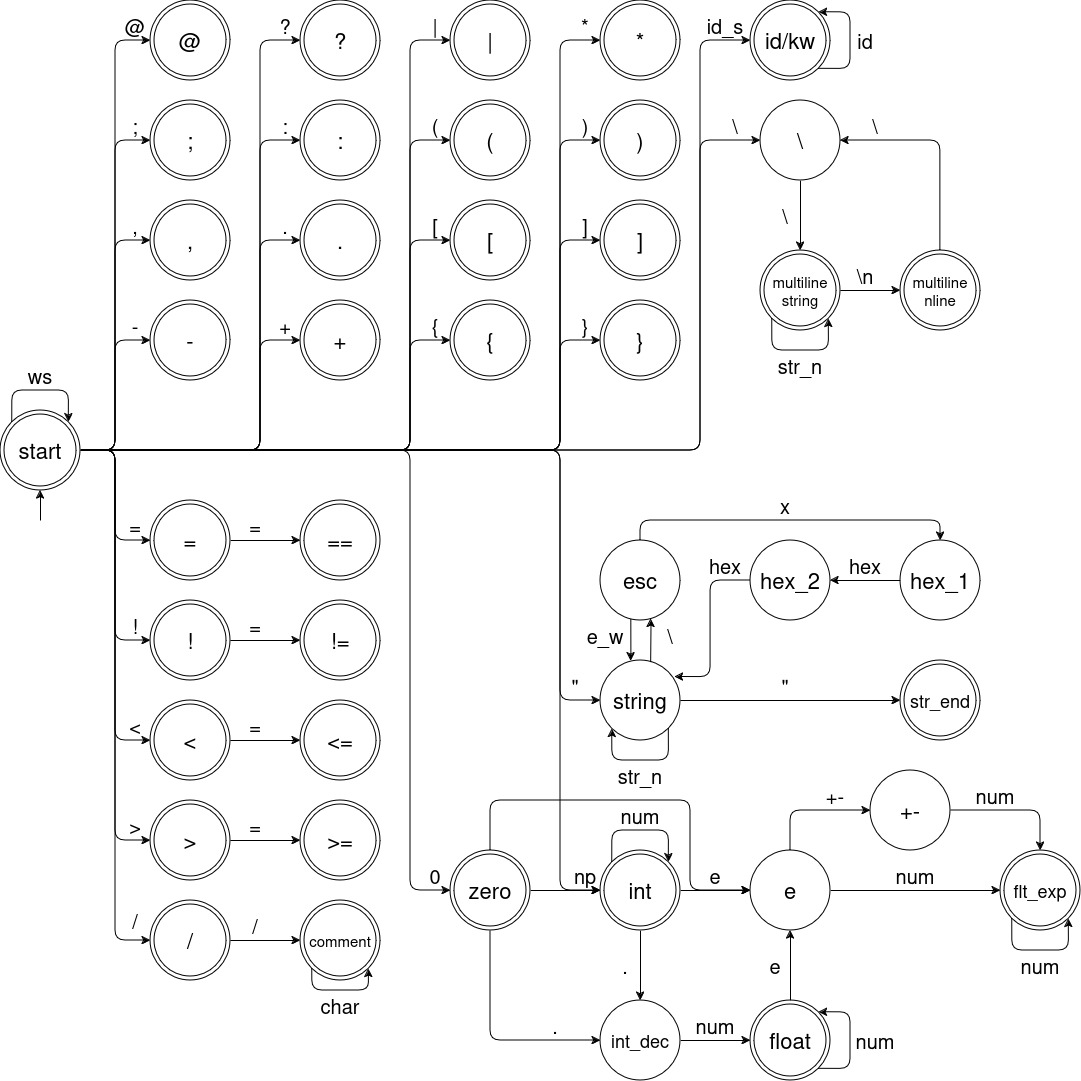
\includegraphics[width=0.8\textwidth,scale=0.5]{fsm}

\newpage

 \Large \textbf{LL-gramatika :} \\ \normalsize
\noindent\makebox[\linewidth]{\rule{\textwidth}{0.4pt}}
\begin{enumerate}
\item aaaa
\item bbbb
\item ccccc
\item ddddddddd
\end{enumerate}


 \Large \textbf{LL-tabulka :}
\newline \\


\includegraphics[width=0.3\textwidth,scale=0.3]{LLtabulka}

 \Large \textbf{Precendecna-tabulka :}
\newline \\


\includegraphics[width=0.3\textwidth,scale=0.3]{Ptabulka}


\newpage

 \Large \textbf{Lexikalna analyza} \normalsize \\
\noindent\makebox[\linewidth]{\rule{\textwidth}{0.4pt}}

\paragraph{\indent Riešenie lexikálnej analýzy sme začali vytvorením diagramu deterministického konečného automatu. Následne sme na jeho základe začali vypracovávať implementáciu. Implementácia sa nachádza v súbore \textit{scanner.c,} ktorý pracuje s tokenmi deklarovanymi v súbore \textit{token.h}. Hlavnou funkciou \textit{scanner.c} je funkcia \textit{get\_token}. Pre uľahčenie práce a prehľadnosti kódu sme si deklarovali niekoľko makier, ktoré sú extensivne používané v hlavnej funkcii. Funkcia \textit{get\_token} berie postupne znaky zo štandardného vstupu a vytvára token. Tokenu je priradeny jeho typ a hodnota, ktorá mu odpovedá. Funkcia začína určovaním jednoznakovych tokenov, ktoré vie určite hneď na začiatku. Pokračuje identifikáciou komentárov, ktoré následne ignoruje. Po identifikácii komentárov zisťuje či sa jedna o ID alebo Keyword, pri kľúčových slovách sa následne určuje aj ich typ. Ak sa nejedna ani o jedno pokračuje kontrolou dátových typov, pri ktorých ukladá aj ich hodnoty.  \newline \\}

 \Large \textbf{Syntakticka analyza}\normalsize \\
\noindent\makebox[\linewidth]{\rule{\textwidth}{0.4pt}}

\paragraph{Riešenie syntaktickej analýzy sme započali vytvorením LL gramatiky, LL tabuľky a precendecnej tabuľky. Následne na ich základe sme vypracovali súbor \textit{parser.c a exp\_parser.c}.Tieto súbory pracujú s uzlami deklarovanymi v súbore \textit{ast.h}. Spustenie syntaktickej analýzy započne zavolanim funkcie \textit{Parse()}. Tato funkcia postupne prechádza cez tokeny a priradzuje ich do uzlov, pomocou ktorých postupne tvorí abstraktný syntakticky strom na základe LL gramatiky. Súbor \textit{parser.c} ďalej riadi aj precedencnu analýzu volaním funkcii zo súboru \textit{exp\_parser.c}. Tento súbor vytvorí strom výrazov, ktorý je následne pripojení do syntaktického stromu.  \newline \\}

 \Large \textbf{Semanticka analyza}\normalsize \\
\noindent\makebox[\linewidth]{\rule{\textwidth}{0.4pt}}

\paragraph{Sémantická analýza je implementovana v súboroch \textit{sem\_anal.c , symtable.c, sem\_anal.h a symtable.h}. Spustenie sémantickej analýzy započne zavolanim funkcie \textit{analyse()}. Sémantická analýza je založená na rekurzivnom prechode AST stromu, ktorý je prevzatí od funkcie \textit{parse()}, ktorá ho vygenerovala. Funkcia ďalej využíva globálne deklarovany AST strom, v ktorom sa nachádzajú built in funkcie. Pri generácií nového AST stromu sa do neho vkladajú built in funkcie práve z tohto globálneho stromu. Funkcia \textit{analyse()} po spustení hľadá \textit{main} a následne postupne rekurzivne prechádza cez AST strom, kde kontroluje validitu dátových typov uložených v ASTNode štruktúrach. Po tejto kontrole započne aj kontrola navratovych hodnôt. Po úspešnej validacii dát predáva nový AST strom funkcii \textit{codegen()}, ktorá začína generaciu kódu. Ak validacia neprebehne úspešne, vyhlási sematicku chybu. \newline \\
Symtable, ktorý tato funkcia využíva je implementovany ako AVL strom.  \newline \\}

 \Large \textbf{Generovanie kodu} \normalsize \\
\noindent\makebox[\linewidth]{\rule{\textwidth}{0.4pt}}

\paragraph{Generátor je implementovany v súboroch \textit{codegen\_priv.h. codegen.h a codegen.c }.Spustenie generácie kódu započne zavolanim funkcie \textit{codegen()}. Kód je generovaný na základe rekurzivneho prechadzania abstraktivneho syntaktického stromu podľa dátového typu uloženého v štruktúre \textit{ASTNode}. Kód ďalej využíva aj pomocný Linked List na ukladanie deklarovanych premenných v danej funkcii. \newline \\}


\newpage

 \Large \textbf{Datove struktury}\normalsize \\
\noindent\makebox[\linewidth]{\rule{\textwidth}{0.4pt}}

\paragraph{\large \underline{Circular Buffer}\normalsize \\ Implementovane v súboroch \textit{circ\_buff.c circ\_buff.h}. \\ \newline
Implementácia Circular Buffer je využitá hlavne v časti Scanner, kde slúži na bezpreblemove získavanie dať a ich následnú validaciu. Na prácu so scannerom ho neskôr využívajú aj časti Parser a Expression Parser. Štruktúra obsahuje klasické funkcie \textit{circ\_buff\_init, circ\_buff\_free, circ\_buff\_enqueue, circ\_buff\_dequeue, circ\_buff\_is\_empty}. 
\newline \\}

\paragraph{\large \underline{Dynamic String}\normalsize \\ Implementovane v súboroch \textit{dyn\_str.c, dyn\_str.h}. \\ \newline
Implementácia dynamického reťazca je využitá hlavne v Scanner časti programu, kde sprostredkuvava validaciu a uschovavanie dať, neskôr je použitá aj v časti Codegen, kde slúži na uľahčenie validacie dať. Štruktúra dynamického reťazca obsahuje klasické funkcie \textit{dyn\_str\_init, dyn\_str\_grow, dyn\_str\_append, dyn\_str\_append\_str a dyn\_str\_free}.  
\newline \\}

\paragraph{\large \underline{Stack}\normalsize \\ Implementovane v súboroch \textit{stack.c, stack.h}. \\ \newline
Implementáciu nášho zásobníku využívame v Expression Parser časti programu. Štruktúra zásobníku je implementovana s klasickými funkciami \textit{stackInit, stackPush, stackPop, stackIsEmpty, stackClear a stackGetTop}. Zásobník sme zvolili pre jeho optimálny prístup k dátam a zachovanie jednoduchosti kódu.
\newline \\}

\end{document}
